% adding the line below for Multifile document support with LatexTools Sublime package 
%!TEX root = manuscript.tex


% Discussion

\section{Discussion}

\subsection{Perform the meta-analysis}
In the meta-analysis performed here, we challenged some choices made by \citeauthor{Cortese2016}, 
which proved controversial: the computation of \gls{es} based on an unusual scale \citep{Steiner2014} and the inclusion 
of a pilot study \citep{Arnold2014} whose final results weren't available at the time \citeauthor{Cortese2016} 
conducted his meta-analysis. We review here the list of changes, their justification, and their impact on the analysis.
 
First, relying on the Conners-3 \citep{Conners2008} instead of the BOSS Classroom Observation \citep{Shapiro2010} 
for teachers ratings seems preferable because this scale is more often used \citep{Christiansen2014, 
Bluschke2016} and is the revision of the Conners Rating Scale Revised \citep{Conners1998} whose reliability has been studied 
\citep{Collett2003}. However, relying on one or the other scale does not 
change the significance of the \gls{es} whatever the outcome studied.

Second, to compute the \gls{es} of \citet{Arnold2014} we used the values at post-test
that is to say when all sessions were completed. Some studies suggest that the number of sessions positively 
correlates with the changes in the \gls{eeg} \citep{Vernon2004} so a lower number of sessions would lead to 
artificially smaller \gls{es}. Here, the \gls{es} computed with the values at post test of \citet{Arnold2014} 
are smaller than those obtained after 12 sessions but these differences do not lead to a change of significance 
of the \gls{se}. 

To conclude on that meta-analysis, though some points from the original were controversial and the fact that 
- for the reasons mentioned earlier - different choices could reasonably be made, 
it turns out that the impact on the meta-analysis results are minimal and do not change the statistical significance of any outcome. 
Consequently, the completion of the meta-analysis with studies published since the publication of his work were done with the choices: 
\begin{itemize} 
	\item to compute the \gls{es} of \citet{Arnold2014} the values at post-test were used;
	\item the scores reported by teachers on the Conners-3 in \citeauthor{Steiner2014}'s study were taken into account instead of these of 
	the BOSS Classroom Observation.
\end{itemize} 

The addition of the two new studies \citep{Strehl2017, Baumeister2016} further confirms those results. Indeed, 
the significance does not change for any outcome: \gls{se} found remains significant for \gls{mprox} raters and 
non-significant for \gls{pblind}. 

Adding two more studies increases the significance of the sensitivity analysis ran by \citeauthor{Cortese2016}, 
most interestingly, the \gls{se} from the subset of studies corresponding to standard protocols of \gls{nfb} as 
defined by \citet{Arns2014}. While \citeauthor{Cortese2016} found that this subset tends to perform better, particularly
on the \gls{pblind} outcome, adding two studies confirms this result on the total clinical score (p-value < 0.05). 
Despite the obvious heterogeneity of the studies included in this subset (particularly in terms of protocol used), 
this result suggests a positive relation between the features of this \emph{standard} design and \gls{nfb} performance.

Eventually, concerning the raters, we considered teachers as \gls{pblind} raters as \citeauthor{Cortese2016} and 
\citeauthor{Micoulaud2014} did although they may be aware of the treatment followed thanks to the parents. 
Besides, the amplitude of the clinical scale at baseline suggests that teachers do not capture the full picture of 
the condition or see it differently and are therefore less likely to see a change (prone to type II error) \citep{Sollie2013, Narad2015}.
So using \gls{pblind} as an estimate for placebo amplitude assessment may be wrong.

Along with this article, the Python code and raw data are provided in order to facilitate a potential replication of this work
(available on the GitHub repository).  

% 573 words

\subsection{Identify factors influencing the Neurofeedback}

Description and analysis of \gls{nfb} implementation was subject to several studies \citep{Arns2014, Enriquez2017, Vernon2004, Jeunet2018} 
but to our knowledge none used statistical tools to detect the influence of methodological, clinical and technical factors 
on such a wide range of studies. 

A somewhat puzzling result is the fact that the three methods which offer to identify factors contributing to the \gls{nfb} 
performance do not lead to the exact same results. These discrepancies are clearly explained by the varying hypothesis 
of these models and actually offer interesting insight into the results and their significance. For instance, the decision tree method is non 
linear and accounts for variables interaction which is not the case for the two others methods. Moreover, the decision tree is unstable 
\citep{dwyer2007}, meaning that a small change in the data can cause an important change in the structure of the optimal decision tree.

Nevertheless, despite these differences between the methods, several factors are selected by at least two methods and among them 3 are
consistently identified by all the methods with the same direction of influence: if the rater is probably blind to the treatment, the
treatment length, and the EEG quality. 

Surprisingly, the number of sessions is not found as a significant influencing factor by any method, 
which is somewhat in contradiction with existing literature. For instance, \citet{Enriquez2017} insisted on the 
fact that the number of sessions should be chosen carefully to avoid "overtraining". Moreover, \citet{Arns2014} stated that 
performing less than 20 \gls{nfb} sessions lead to smaller effects. Indeed \citet{Vernon2004} observed that positive 
changes in the \gls{eeg} and behavioral performance occurred after a minimum of 20 sessions, but he also points out the fact that the
location of the \gls{nfb} training may had an important influence. Nevertheless, in our study, regardless of the significance of 
the number of sessions, the coefficient found by the \gls{wls} is negative, meaning that as expected,
the more sessions performed the more efficient the \gls{nfb} seems to be. 

The type of protocol is not identified by all the three methods but it seems to influence the \gls{nfb} results according to 2 methods,  
in particular the theta down protocol which appears more efficient and \gls{smr} protocol which conversely seems associated with lower \gls{es}. We expected 
more precised results on the protocols criteria because this point is central in \gls{nfb} as pointed out by \citet{Vernon2004}.
A possible explanation is that all these protocols are equally efficacious to the populations they were offered to and 
thereby do not constitute a significant explanatory factor. This result, however, does not preclude a combined and personalized strategy 
(offer the right protocol to the right kid) to further improve performance. 

As precised earlier, the three methods agree on three factors.

First, this analysis points out the fact that recording \gls{eeg} in good conditions seems to lead to better results, 
which can be explained by the fact that better signal quality enables to extract more correctly the \gls{eeg} 
patterns linked to \gls{adhd} and henceforth leads to better learning and therapeutic efficacy. However, it remains difficult to 
really assess the quality of the hardware because little information is provided in the studies.  

Next, it appears here that the longer the treatment the less efficient it becomes. Arguably, the treatment length is a proxy 
for treatment intensity, which means that a treatment that is short in length (and consequently intense in pace) 
is more likely to succeed. This hypothesis is back-up by the fact that the variable \emph{session pace} (number of sessions per week) 
is also associated with larger \gls{es} according to the \gls{wls} and \gls{lasso}. 

As expected, the assessment of symptoms by non-blind raters leads to more favorable results than by \gls{pblind} raters - 
result observed in several meta-analysis \citep{Cortese2016, Micoulaud2014}. 

We decided to investigate more precisely this factor, in order to determine if this observation can be solely explained by
the placebo effect. First, to assess the impact of the placebo effect, we rely on the results of the decision tree 
presented in \cref{Figure:factors_analysis_decision_tree_results} which splits the dataset in two subsets: on one hand 43 observations corresponding 
to \gls{mprox} raters assessments and on the other hand 19 observations corresponding to \gls{pblind}. If the differences observed 
between \gls{pblind} and \gls{mprox} raters are due to the placebo effect, we can expect to find in the \gls{mprox} part of the decision 
tree factors linked to the perception of the treatment. It is, indeed the case: session and treatment length are returned but if
these factors are really linked to the placebo effect, we can expect that the longer the session and the treatment, the higher the \gls{es}. 
Yet, we observe the opposite: it is not in favor of the presence of the placebo effect. 

Another way to highlight a possible placebo effect, is to focus on the difference between \gls{pblind} and \gls{mprox} raters first at pre-test 
and then at post-test. The differences of ratings between teachers and parents have been prone to different studies \citep{Sollie2013, Narad2015}
which note that teachers are more susceptible to give lower scores especially on younger children. We also observe that fact on most of the studies included 
in our analysis as illustrated in \cref{Figure:discussion_on_placebo_effect_colors_2-columns_fitting_image}.  

\begin{figure}[h!]
  \centering
  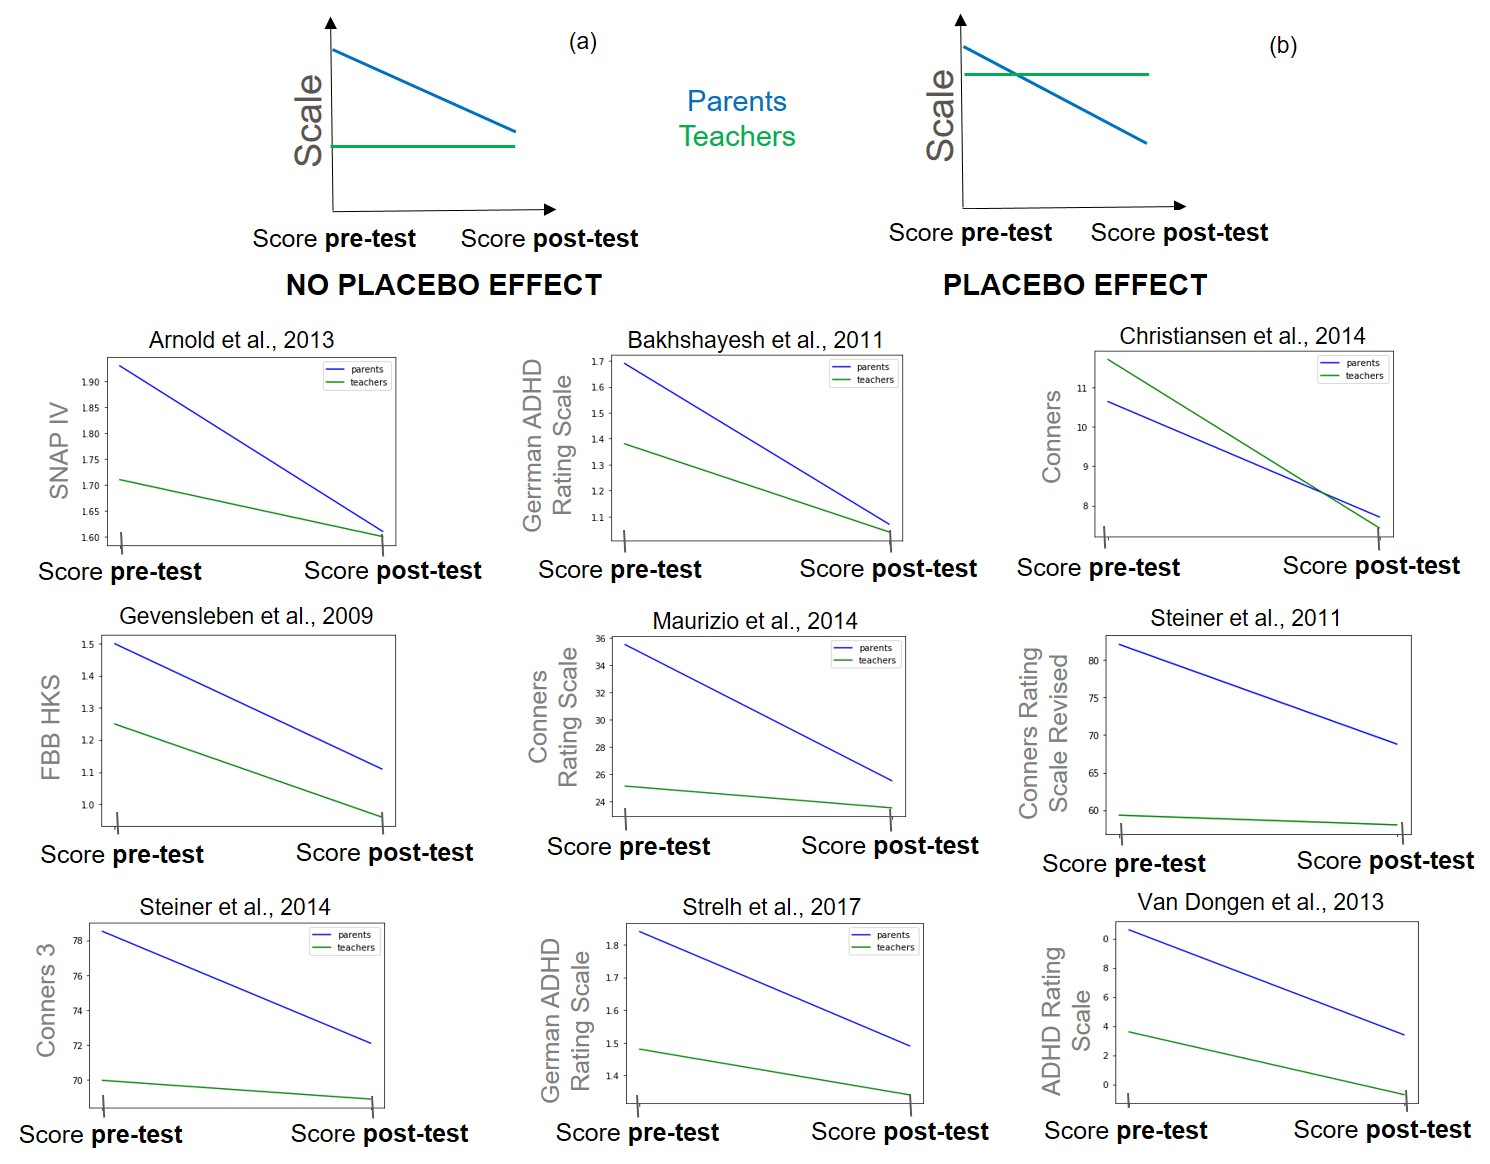
\includegraphics[width=1.0\linewidth]{figures/discussion_on_placebo_effect_colors_2-columns_fitting_image}
  \caption{Pre-test and post-test scores ($\pm$ standard error) given by Parents (\gls{mprox}) in blue and teachers (\gls{pblind}) in green. Two configurations: (a) teachers don’t see the symptoms at 
	pre-test so they can’t see any improvement at post-test, (b) teachers see the symptoms at pre-test and don’t see any improvement at post-test. (c) Evolution of parents and teachers' scores
	between pre and post-test on studies that satisfy \citeauthor{Cortese2016}'s inclusion criteria and that provide teachers and parents scores on the same scale.}
  \label{Figure:discussion_on_placebo_effect_colors_2-columns_fitting_image}
\end{figure} 

Thus, these results suggest that \gls{pblind} assessments can hardly be used to assess placebo as they seem to be more blind
to symptoms rather than to intervention. In the absence of ethically and technically feasible sham \gls{nfb} protocols, it seems preferable 
that evidence of control, learning, and specific changes (correlation with symptoms) are used to determine the mode of action further 
(neuromarker analysis).      

It would have been interesting to study the influence of some other factors such as the delay between brain state and feedback 
signal as well as the type of \gls{nfb} game used, but these information are rarely available in studies. Besides, 
to add more reliability to these results it should be preferable to add more studies, 
particularly studies with teachers assessments (considered as \gls{pblind}). 

% words number = 849
